\section{Effect of Grid Storage} \label{sec:res-storage}

In section \ref{sec:grid-implementations}, we described different approaches to storing an unstructured grid. Four storage approaches were benchmarked as a result of varying the following two properties: First, the depth of the neighborship table, i.e. whether only neighbors (\emph{chasing} variant) or also neighbors-of-neighbors (\emph{non-chasing} variant) were stored. Second, whether the neighborship table was \emph{compressed} or \emph{uncompressed}.

\begin{figure}
	% ax=u.barplot(df64mins[(df64mins["stencil"]=="hdiff")&df64mins["z-curves"]&(df64mins["size-x"]>=128)], grp=u.col.stencil+u.col.size, cat=u.col.storage, tickrot=0, y="rel")
	% ax.set_ylim(bottom=1)
	% fig=u.plotdone()
	% u.plotsave("report/img/hdiff-z-curves-sizes-storage.pdf", fig)
	\comment{
	      stencil  size-x  size-y  size-z  unstructured        variant  z-curves  no-chase   comp  threads-x  threads-y  threads-z       min       max       avg    median
	11327   hdiff     128     128      64          True         idxvar      True     False  False         64          1          8   50000.0   53000.0   51000.0   51000.0
	12079   hdiff     128     128      64          True         idxvar      True     False   True         32          1         16   52000.0   56000.0   53000.0   53000.0
	10516   hdiff     128     128      64          True         idxvar      True      True  False         32          2          8   47000.0   50000.0   48000.0   49000.0
	10880   hdiff     128     128      64          True          naive      True      True   True         32          1          8   48000.0   51000.0   50000.0   50000.0
	32073   hdiff     512     512      64          True         idxvar      True     False  False         64          1          8  801000.0  828000.0  817000.0  820000.0
	31623   hdiff     512     512      64          True         idxvar      True     False   True        128          1          2  734000.0  746000.0  741000.0  741000.0
	32178   hdiff     512     512      64          True  idxvar-shared      True      True  False         32          1         16  819000.0  854000.0  838000.0  841000.0
	31541   hdiff     512     512      64          True          naive      True      True   True        128          1          2  707000.0  721000.0  713000.0  710000.0
	}
	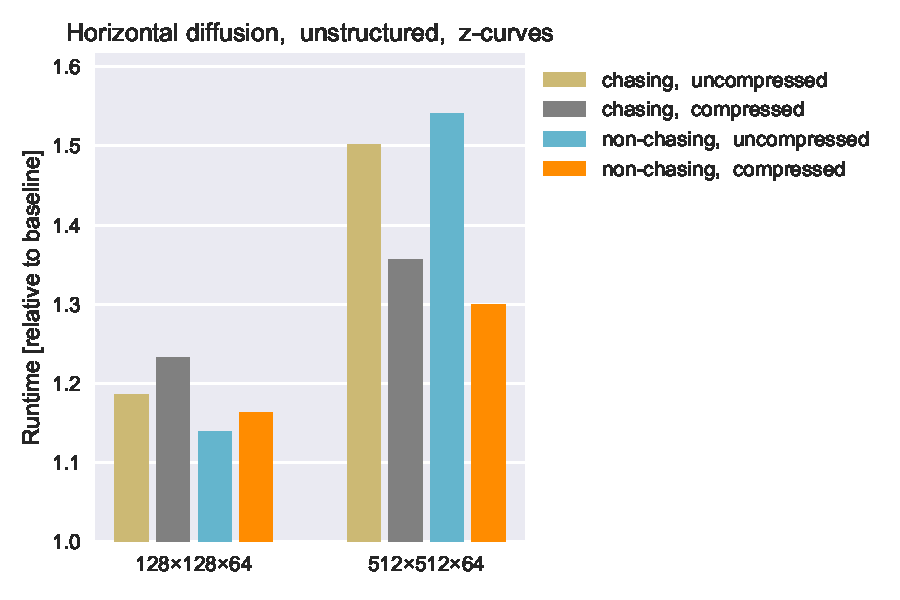
\includegraphics[scale=0.75]{hdiff-z-curves-sizes-storage.pdf}
	\caption{\label{fig:hdiff-sizes-storage} Relative slowdowns for the horizontal diffusion stencil on a small and a larger grid. The fastest access variant is plotted for each bar, which is one of \emph{index variables}, \emph{naive} and \emph{idxvar-shared} for the shown benchmarks. This example for the horizontal diffusion stencil is representative for the other two benchmarks as well, where the slowdowns follow a similar pattern. (Note that in the fastwaves stencils, pointer chasing is not applicable as there only direct neighbors are accessed.) Baseline: fastest regular grid implementation.}
\end{figure}

\subsection{Pointer Chasing vs. Neighbor-of-Neighbor Storage}
\label{sec:results-chasing}

Two of the three benchmarked stencils, Laplace-of-Laplace and Horizontal Diffusion, access neighbors beyond the directly face-touching cells (neighbors of neighbors). For those stencils, two implementations were benchmarked: First, we assessed the performance when only direct neighbors are explicitly stored. This approach requires \emph{pointer chasing}: In order to access the neighbor of a neighbor, two sequential lookups become necessary. As the second lookup can only be started when the first one completed, a higher latency may occur in this variant. Therefore, we then also tested variants in which the neighbors-of-neighbors were explicitly stored in memory, reducing the number of required memory lookups for those cells from two to one. This comes at the cost of a higher memory footprint, however.

Generally we observe the following trend: If the grid is small or compressed, pointer chasing becomes an issue (and thus non-chasing variants profit). In larger uncompressed grids, the latency of the two lookups required in pointer chasing for neighbors-of-neighbors can be effectively hidden. This is visible in figure \ref{fig:hdiff-sizes-storage}, which outlines the differences of the storage approaches for the fastest respective variant of the horizontal diffusion stencil on grids of different sizes. 

In all cases a higher total number of device memory and L2 cache reads is observed in the \texttt{nvprof} metrics for the non-chasing variants. This is to be expected, as non-chasing variants need to store and read more information from a larger number of different addresses. The L1 cache hit rate lowers by around $6\%$ in both large and small grids when pointers to neighbors-of-neighbors are explicitly stored. In large grids, the L2 cache hit rate also drops dramatically; for smaller grids, it is unaffected and remains high. Thus, the additional neighbor-of-neighbor information stored hurts cache locality more in larger grids, putting non-chasing variants at a disadvantage there. This is due to the fact that larger grids require more of this information, while the cache size remains constant -- consequently, some data has to be evicted from the cache. This does not happen as often in a smaller grid. The variants that perform pointer chasing experience a higher percentage of stalls due to memory dependencies due to the second lookup depending on the result of the first for neighbor-of-neighbor reads.  We conclude that non-chasing storage is beneficial to small grids, where it is effective in reducing latency, and unfavorable for larger grids due to the caused cache evictions (especially in the L2 cache), that actually increase the latency of neighbor acceses. Table \ref{tab:chasing} shows an overview of the metrics discussed in this paragraph for an exemplary stencil configuration of the horizontal diffusion stencil.

\begin{table}
	\comment{chase-v-no-chase.txt}
	\begin{tabular}{l c p{1.5cm} p{1.5cm} p{2.5cm} l}
		\hline
		\textbf{Size} & \textbf{Chasing?} & \textbf{\texttt{tex\_\allowbreak cache\_\allowbreak hit\_\allowbreak rate}} & \textbf{\texttt{l2\_\allowbreak tex\_\allowbreak hit\_\allowbreak rate}} & \textbf{\texttt{stall\_\allowbreak memory\_\allowbreak dependency}} & \textbf{Runtime} \\
		\hline
		\hline
		$128\times 128\times 64$ & - & 			$73\%$ & $68\%$ & $59\%$ & $\mu s$ \\
		$128\times 128\times 64$ & \checkmark & $67\%$ & $72\%$ & $54\%$ & $\mu s$ \\
		\hline
		$512\times 512\times 64$ & - & 			$68\%$ & $58\%$ & $74\%$ & $\mu s$ \\
		$512\times 512\times 64$ & \checkmark & $63\%$ & $37\%$ & $60\%$ & $\mu s$ \\
		\hline
	\end{tabular}
	\caption{\label{tab:chasing} Selected metrics for runs of the horizontal diffusion stencil on different types of grids (all of them in z-curves layout). The fastest found variant and launch configuration was chosen for each configuration seperately.}
\end{table}

\subsection{Effect of Neighborship Table Compression}

In section \ref{sec:compression}, we described a very simple compression scheme for the neighborship table. Using this scheme, cells with the same neighbor offsets can ``share'' their neighborship table entries. Table \ref{tab:compression} shows the distribution of neighborship table entries (patterns) attained on a $512\times 512\times 64$-sized grid for the two value memory layouts benchmarked (\emph{row-major}, \emph{z-curves}). If the values of the grid are laid out in row-major fashion, the number of distinct patterns is lowest. In this case, only the elements in the halo have different neighborship pointers; all others share the top entry. Using a z-curves layout, the distribution of neighborship table accesses is more spread out. However, the concentration of several frequently occuring patterns is still able to provide a runtime benefit.

\begin{table}
	\begin{tabular}{l l l l l l}
		\hline
		Compressed? & Chasing? & Storage & \# Entries & Ratio\textsuperscript{*} & Freq.\textsuperscript{\dag} \\
		\hline
		- & \checkmark & both & $1,048,576$ & $1$ & $<1\%$\\
		- & - & both & $3,145,728$ & $1$ & $<1\%$\\
		\checkmark & \checkmark & row-major & $2054$ & $0.00078$ & $97.7\%$ \\
		\checkmark & \checkmark & z-curves & $2435$ & $0.00093$ & $20.3\%$ \\
		\checkmark & - & row-major & $4093$ & $0.00156$ & $96.9\%$ \\
		\checkmark & - & z-curves & $5299$ & $0.00202$ & $8.1\%$ \\
		\hline
	\end{tabular}
	\caption{\label{tab:compression} Properties of neighborship table before and after compression for different types of grids. \textsuperscript{*}Ratio of number of compressed neighborship table entries to number of uncompressed neighborship table entries. \textsuperscript{\dag}The frequency given is the frequency of the most common neighborship table entry. }
\end{table}

In large grids, across all stencils except \emph{fastwaves}, and for all access strategies, compressing the neighborship table improves performance. We observe a reduced number of device memory reads when compressed storage is used, proving the efficacy of the compression scheme.

% mention coalescing worsens
% mention that block size has to be right; for 64x1x4, idxvar is faster (z-curves); similar argument to below for small grids (if we have repeating z-levels, then direct caching of neighborship pointer is faster than additional pointer chase through patterns array; compressed gets its speed from the fact that we can use block sizes that are more natural for the VALUES of the grid, i.e. 256x1x1 block size to read many values at once)

In small grids, compression is not beneficial. This can also be seen in figure \ref{fig:hdiff-sizes-storage}. We assume that in small grids, neighborship information fits into the caches. % small grids: pattern lookup another "hoop to jump through"; after first Z-level, neighborship pointers in cache anyways; this is evidenced by the fact that for 128x128x1, compressed is faster again (slightly; pattern is in cache then after first cell; no advantage of cache for multiple z-levels as there is only one)

\begin{verbatim}
% TODO
% - Relative advantage of compression for all variants/combinations
% - Why not larger advantage? -> Metrics to back up coalescing explanation/latency of first prototype lookup and second lookup is non-coalesced
% - Why uncompressed faster for fastwaves?

% mention fewer memory dram transactions/bytes in compressed variants
% mention higher hit rate for large grids, smaller hit rate for small
\end{verbatim}
